\documentclass{./class/itisreport}
\DocuMetadata{
    Title={Validation of Pattern Assessment Software for Use in SAR Measurement System Validation (Version 2)},
    HeadTitle={Validation of Pattern Assessment Software},% if this is empty, the Title is used in the header
    Conducted={Javier Ordonez, Melanie Steiner, Matthew Morvan, Esra Neufeld, Alessandro Fasse, Mark Douglas, Niels Kuster},
    Date={\today},
    %Disclaimer={},% In case you want to change the default
    %Confidential={},% In case you want to change the default
    Project={1464},
    DocuName={STD-1464},
    Rev={1},
    AutName={Mark Douglas},
    AutFunction={Project Leader,\hspace{15mm}IT'IS Foundation},
    AutDate={},% leave blank, will be filled with DocuSign
    AppName={Niels Kuster},
    AppFunction={Quality Manager,\hspace{15mm}IT’IS Foundation},
    AppDate={},% leave blank, will be filled with DocuSign
    Customer={Customer Name},
    Watermark={DRAFT}
}
\SetWatermarkColor[gray]{0.95}
\SetWatermarkScale{0.6}

%if you want to print it, this adds a blank page between the signature page and the cover page
\newbool{print} % it is initially set to `false' and can be changed by commenting below
\booltrue{print}
\boolfalse{print}

% Useful packages
\usepackage[english]{babel}
% \usepackage[a4paper,top=2cm,bottom=2cm,left=3cm,right=3cm,marginparwidth=1.75cm]{geometry}
\usepackage{amsmath}
\usepackage{amssymb}
\usepackage{graphicx}
\usepackage{subcaption}
\usepackage{placeins}
% \usepackage{subfigure}
\IfFileExists{biblatex.sty}{%
  \usepackage[sorting=none]{biblatex}%
  \addbibresource{bib.bib}%
}{%
  \newcommand{\printbibliography}{\bibliographystyle{IEEE}\bibliography{bib}}%
}
\usepackage{dcolumn}
\newcommand{\git}{https://github.com/ITISFoundation/SAR-Pattern-Validation}

\begin{document}

\section*{Revision History \label{sec:revision}}
\subsection*{Revision 1}
\begin{itemize}
    \item Revised according to the input received by the standard group
\end{itemize}
\subsection*{Revision 0}
\begin{itemize}
    \item Initial version of Zurich, 21 March 2026 presented at the IEC Meeting in Vienna.
\end{itemize}
\clearpage

\section*{Executive Summary \label{sec:exec_summary}}

Validation of spatial SAR distributions was proposed as a way to strengthen the validation of SAR measurement systems. The Gamma comparison method was proposed, based on its use in other fields, its ease of implementation, and its ability to compare distributions with positioning and co-registration uncertainties. Evaluation of the full SAR distribution, not just at the peak location, improves the detection of any system non-compliance and improves the efficiency of the validation.

A reference implementation of the approach has been provided. The code was developed by the Foundation for Research on Information Technologies in Society (IT'IS). It can be found, along with full documentation, a tutorial and validation scripts, on a \href{\git}{GitHub repository}. This document describes that reference implementation and its verification. 

The user uploads a measured SAR distribution and chooses the input parameters (antenna type, frequency, distance, averaging mass).
The code evaluates the Gamma match and determines whether the sSAR distribution is compliant, according to the criteria. The software also creates plots to show the measured and reference SAR distributions, the registration overlay, the gamma index map and the pass/fail map.

This document is divided into three parts:

\begin{itemize}
\item Background and Objectives (Section~\ref{sec:objectives}) provides a brief history of SAR validation in IEC and IEEE standards, introduces pattern matching, and describes the implementation and parameters;
\item Sampling Software (Section~\ref{sec:method}) describing the use and operation of the software;
\item Validation (Section~\ref{sec:val-all}) describing efforts undertaken to ensure functionality, correctness, documentation, and expected behavior; this involved the following validation activities:
\begin{itemize}
\item code testing (Section \ref{sec:code-val}): ensuring that the mathematical and behavioral properties expected from the software are satisfied;
\item code review (Section \ref{sec:code-review}): review of the code by an otherwise uninvolved developer for additional quality assurance;
\item functional testing (Section \ref{sec:func-test}): end-to-end testing of the overall implementation to ensure that the desired behavior is satisfied.
\end{itemize}
\end{itemize}

The code has been fully validated for use. The results presented in this report demonstrate that the reference implementation satisfies the expected mathematical properties and provides usable results in the desired form.

\tableofcontents

\clearpage
\FloatBarrier
\section{Background and Objectives \label{sec:objectives}}


\subsection{History of SAR Validation} \label{sec:history}

IEEE 1528-2003 was the first standard that included validation of SAR measurement systems. This standard was written for single-probe scanning systems, and the validation consisted of a fixed set of tests. This validation is considered to be robust, given that each component of the SAR measurement system can be validated independently.

IEC 62209-3:2019 was the first standard applicable for SAR array systems -- systems that are used to evaluate the absolute SAR level. This standard extended the fixed-set validation concept of IEEE 1528-2003 and later standards. It prescribes an unchanging set of test configurations to be measured, typically by the system manufacturer, with every SAR measurement system under test. However, an unoptimized, sparse, and fixed validation sample-set risks insufficient validation space coverage, resulting in low confidence in the validation approach~\cite{bujard2024}. The high degrees-of-freedom of the validation space, and the large ranges of some validation dimensions, result in millions of test conditions to fully cover the validation space with a configuration grid.

IEC/IEEE PAS 62209-5 is now under development to specifically address SAR measurement validation.
To address the limitations of IEC 62209-3:2019, the use of stochastic sampling has been proposed. A Latin-Hypercube sampling (LHS) method has been proposed in a published paper by Bujard et al.\cite{bujard2024}. A code implementation of LHS has been created, as described in a report by the IT'IS Foundation~\cite{lhsreport_2025}. The code outputs a CSV text file that can be used by the testing lab. These test configurations are then measured by the user, and the SAR values are compared to numerical targets using the relevant acceptance criteria to determine if the SAR measurement system is considered validated.

Validation of spatial SAR distributions was proposed as a way to further strengthen the validation of SAR measurement systems. Evaluation of the full SAR distribution, not just at the peak location, improves the detection of any system non-compliance and improves the efficiency of the validation. This has the benefit that it can further reduce the number of tests for the validation.

\subsection{The Gamma Method} \label{sec:g-intro}

We propose an implementation of the Gamma method developed by Low and Dempsey~\cite{low-dempsey} to compare measured spatial SAR distributions, $sSAR_{en}(x_e,y_e)$, with corresponding reference distributions, $sSAR_{rn}(x_r,y_r)$, each normalized to its peak value. The method has been applied previously in the context of validating the agreement between simulated and measured data, taking into account positioning, measurement, and modelling uncertainties~\cite{neufeld2016}. The Gamma method combines two criteria, SAR magnitude difference and spatial distance-to-agreement, combining these two dimensions (after normalization by their respective tolerances $\Delta D$ and $\Delta d$) into a single Euclidian distance norm, $\Gamma$, which is used to identify corresponding points: 

\begin{equation}
\Gamma (x'_e, y'_e) = \min_{x_r,y_r}\Bigg(\sqrt{\frac{(x'_e-x_r)^2+(y'_e-y_r)^2}{\Delta d^2}+\frac{(sSAR_{en}(x'_e,y'_e)-sSAR_{rn}(x_r,y_r))^2}{\Delta D^2}}\Bigg)
\end{equation}\label{eq:gamma}

$sSARen(x_e,y_e)$ and $sSARrn(x_r,y_r)$ are both extracted at the boundary between the phantom shell and lossy medium. Before normalization, masking is performed to select only those values above 0.1 W/kg or twice the noise floor of the system, whichever is lower. A rigid transformation is first applied to the evaluated coordinates ($x_e$, $y_e$) to get the registered coordinates ($x'_e$, $y'_e$) on a 1~mm regular grid that optimally matches the evaluated distribution to the reference distribution. For each point ($x'_e$, $y'_e$) on $sSAR_{en}$, all points ($x_r$, $y_r$) are searched to identify the corresponding point with the minimal Gamma index of Equation~\ref{eq:gamma}. The validation is considered successful if $\Gamma (x'_e,y'_e)~\leq~1.0$ for all points. 


\clearpage
\FloatBarrier
\section{Software \label{sec:method}}

\subsection{Requirements}

The software uses measured spatial-average SAR (sSAR) distributions of validation antennas that are exported by the SAR measurement software. The sSAR must be exported on a rectilinear grid in the ($x$, $y$) plane. Each sSAR distribution must be a comma separated value (CSV) file that is organized into three columns ($x$, $y$ and $sSAR$) as shown in Figure~\ref{fig:csv-file}. Any additional columns will be ignored. The $x$ column header must have an `x' in it, and the $y$ column header must have a `y'. The $x$ and $y$ units are assumed to be in meters unless the column headers include `mm', in which case millimeters will be used.

\begin{figure}[htbp]\centering
\frame{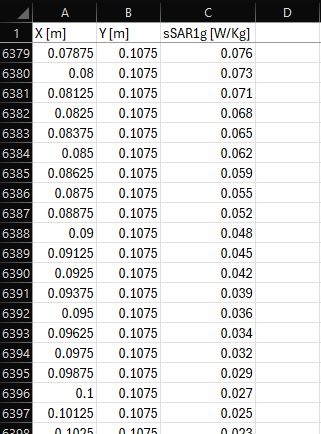
\includegraphics[width=0.4\linewidth]{figs/csv-file.png}}
\caption{Exported CSV file from the SAR measurement software.}\label{fig:csv-file}
\end{figure}

The software includes a database of reference sSAR distributions for each antenna configuration. These have been generated from numerical simulations and exported on a fine grid. There is no need to import the numerical sSAR distribution in the software.

\subsection{Graphical User Interface}

A graphical user interface of the code is publicly accessible on \verb|https://osparc.io/|. Select the project "Pattern Matching Validation". The user interface will look as shown in Figure~\ref{fig:gui-unfilled}.

\begin{figure}[htpb]\centering
\frame{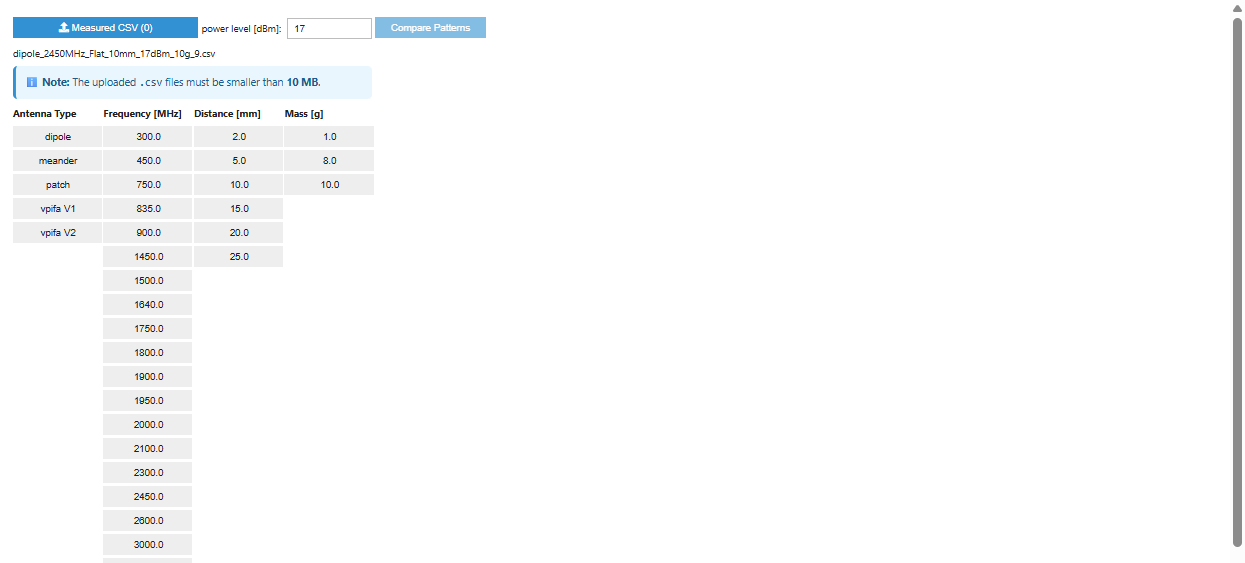
\includegraphics[width=\linewidth]{figs/gui-unfilled.png}}
\caption{Graphical user interface on startup.}\label{fig:gui-unfilled}
\end{figure}

Follow these steps to run the user interface:
\begin{enumerate}
\item Click the button \verb|Measured CSV|.
\item Import the CSV file containing the sSAR distribution of the validation antenna. When this is done, the button will show a `(1)' and the name of the imported file will be shown below the button.
\item Enter the power level that was used for the antenna measurement, in dBm.
\item Select the parameters of the reference sSAR distribution using the selection buttons:
    \begin{itemize}
    \item antenna type
    \item frequency (MHz)
    \item distance (mm)
    \item averaging mass (grams)
    \end{itemize}
\item Click the button \verb|Compare Patterns|
\end{enumerate}

After post-processing, the software runs the Gamma method and populates the plots and values as shown in Figure~\ref{fig:gui-filled}.

\begin{figure}[htpb]\centering
\frame{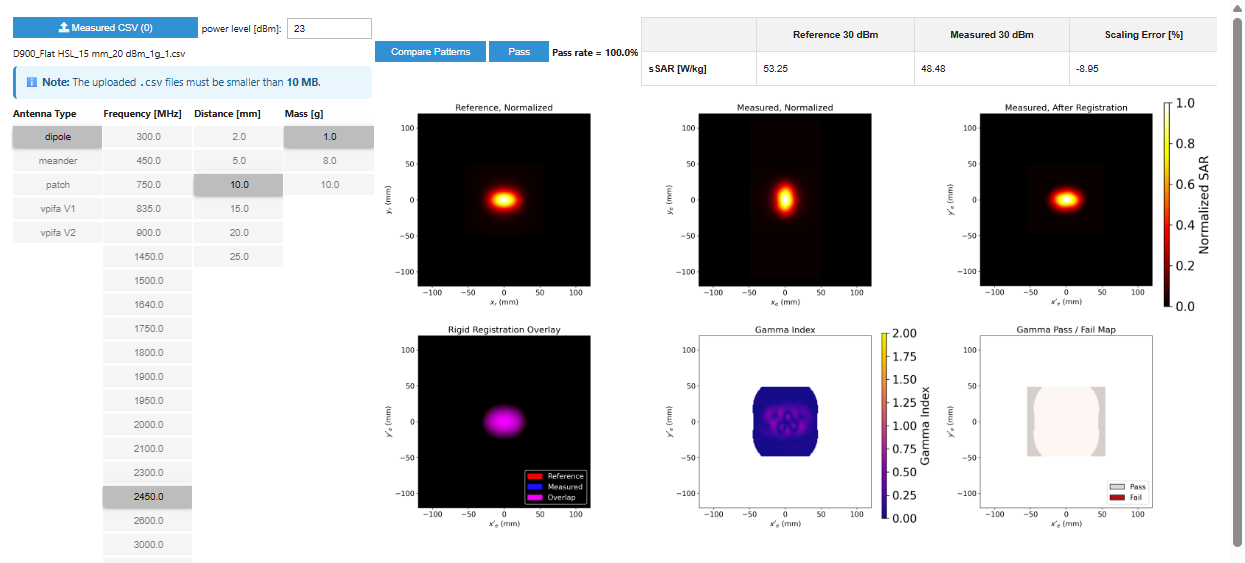
\includegraphics[width=\linewidth]{figs/gui-filled.png}}
\caption{Graphical user interface after selecting `Compare Patterns'.}\label{fig:gui-filled}
\end{figure}

The results, from top-left to bottom right, are:
\begin{itemize}
\item Pass or Fail statement next to the button \verb|Compare Patterns|. The pattern validation passes if $\Gamma~\leq~1$ at all points of the measured sSAR distribution.
\item Pass rate: the percentage of points of the measured sSAR distribution where  $\Gamma ~\leq~1$.
\item Table showing the psSAR of the reference and measured distributions (each normalized to 1~Watt power) and the scaling error (percent difference between the two).
\item Reference sSAR distribution, normalized to the peak value.
\item Measured sSAR distribution, normalized to the peak value.
\item Measured sSAR distribution after registration to match the reference sSAR distribution.
\item Rigid registration overlay, showing the amount of overlap of the measured and reference sSAR distributions after registration.
\item Calculation of the Gamma index (see Equation~\ref{eq:gamma}) at each point of the measured sSAR distribution.
\item Gamma pass/fail map at each point of the measured sSAR distribution. Passing values have $\Gamma~\leq~1$, and failing values have $\Gamma > 1$.
\end{itemize}


\FloatBarrier
\subsection{Source Code}

The source code is available on a public GitHub repository. This code can be downloaded and run without using the graphical user interface. The software operation is the same. It accepts the same inputs and produces the same outputs. 

This section describes how to install the reference implementation and how to run the example. It also describes the organization of the underlying code.

\subsubsection{Tutorial}

A detailed tutorial, showing the function of the code and step-by-step operation, can be found on the GitHub repository by opening the Python Notebook  \verb|tutorial_gamma_comparison_notebook.ipynb|.

\subsubsection{Local Installation}

The software can be installed on your PC as follows (see also the README.md file on the \href{\git}{GitHub repository}):

\begin{itemize}
\item Open a terminal window, for example, Windows PowerShell, or a Unix window, or a terminal window in your preferred IDE (integrated development environment).
\item Go to the folder where you want the software installed.
\item Run the following command in the terminal window:\\ \\
\verb|git clone| \git \\ \\
Alternatively (e.g., if \verb|git| is unavailable), download and extract the Zip file from the \href{\git}{GitHub repository}, as shown in Figure~\ref{fig:download}. Move this file to the folder where you want the software installed, and unzip it.
\item Go to the subfolder SAR-Pattern-Validation.
\item Run the following command: \\ \\ \verb|pip install .| \\ \\
Python and pip dependencies will be handled by the installation process.
\end{itemize}

\begin{figure}\centering
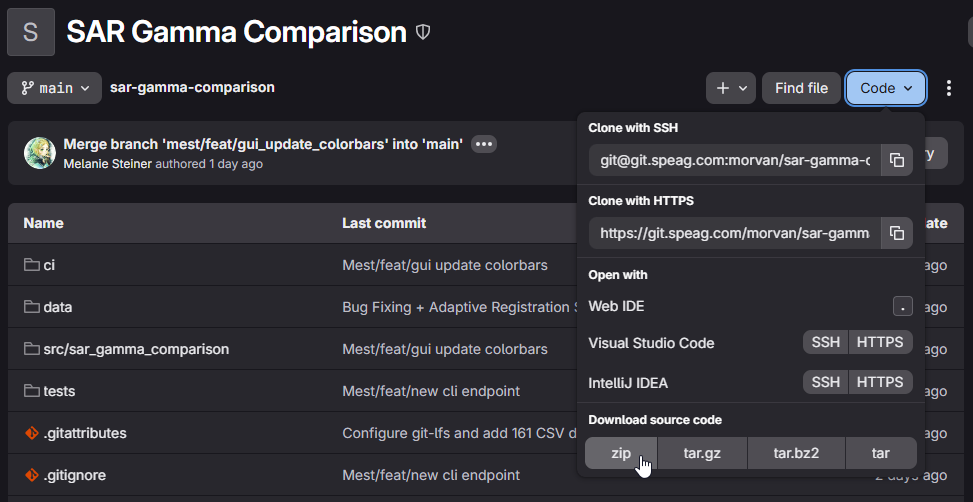
\includegraphics[width=0.7\linewidth]{figs/download.png}
\caption{To download the software to a zip file, click the `Code' button, then select `zip' in the `Download source code' section.}\label{fig:download}
\end{figure}

To check that the code is installed and all Python libraries are installed, run the file \verb|run_pipeline.py|. This uses an example measured sSAR distribution that is provided with the distribution. All plots and outputs will be generated in the results folder.

\begin{figure}[htbp]\centering
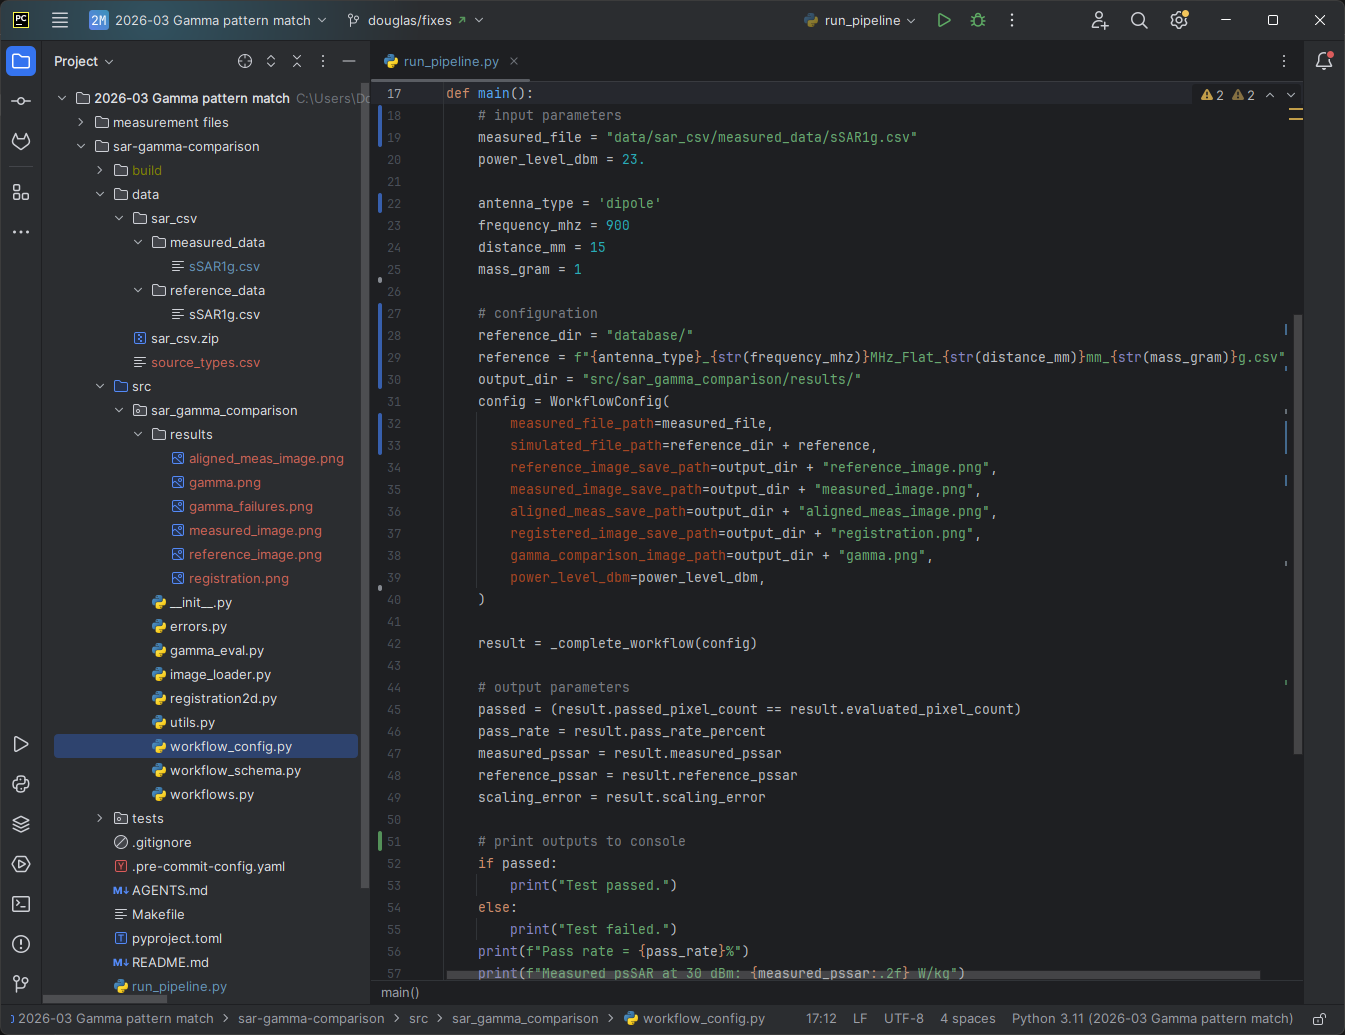
\includegraphics[width=0.9\linewidth]{figs/run_pipeline.png}
\caption{Example file run\_pipeline.py.}\label{fig:run_pipeline}
\end{figure}

The code in \verb|run_pipeline.py| is organized into 4 sections: 
\begin{itemize}
    \item Definition of the six input parameters: 
    \begin{itemize}
        \item two measurement distribution parameters: \verb|measured_file| and \verb|power_level_dbm|
        \item four reference distribution parameters: \verb|antenna_type|, \verb|frequency_mhz|, \verb|distance_mm|, and\\ \verb|mass_gram|
    \end{itemize}
    Note: It is recommended to make a copy of this file if you wish to modify these parameters.
    \item Definition of the configuration, and running the workflow. This creates all of the plots in the results folder.
    \item Extraction of the numerical output parameters.
    \item Printing of the numerical outputs to the console.
\end{itemize}

\FloatBarrier
\subsubsection{Code Description}\label{sec:description}

The sampler code is written in Python (version 3.10 or higher) and consists of five main files:

\begin{itemize}
\item \verb|workflow_config.py|: Defines the parameters of the Gamma match and registration, including $\Delta D$ and $\Delta d$ of Equation~\ref{eq:gamma}, the sample resolution, and the noise floor. It also includes the locations of the input and output files.
\item \verb|workflows.py|: Runs the three steps of the code:
    \begin{enumerate}
    \item Reads the sSAR distributions using \verb|image_loader.py|.
    \item Perform the registration using \verb|registration2d.py|.
    \item Perform the Gamma match using \verb|gamma_eval.py|.
    \end{enumerate}
\item \verb|image_loader.py|: Reads measured and reference sSAR distributions from CSV files, builds 2D grids, and produces images suitable for registration and gamma evaluation.
\item \verb|registration2d.py|: Performs the rigid registration (translation and rotation) of the measured sSAR distribution to match the reference sSAR distribution. Also creates the registration overlay plot.
\item \verb|gamma_eval.py|: Performs the Gamma match of Equation~\ref{eq:gamma} and plots the result.
\end{itemize}

\FloatBarrier
\newpage
\section{Validation}\label{sec:val-all}

Code validation and quality assurance was performed in three steps:

\begin{itemize}
\item \textbf{Code testing:} (Section~\ref{sec:code-val}): internal checks written by the code developer that check that the code functions and that results satisfy the expected mathematical behavior (e.g., for LHS); these checks are implemented in the files \verb|test_lhs.py|, \verb|test_voronoi.py|,
\verb|test_sarsampler.py|, and \verb|test_sample.py|, such that they can easily be (re-)executed.
\item \textbf{Code quality review} (Section~\ref{sec:code-review}): peer review of the code, checking the formal correctness, clarity, suitability of documentation, and ease-of-use.
\item \textbf{Functional testing} (Section~\ref{sec:func-test}): a set of tests to ensure that software outputs match the expected results, without assuming any knowledge about implementation details.
\end{itemize}

\subsection{Code Testing}\label{sec:code-val}

This section lists the tests that have been implemented and executed to verify the functionality of the code.

\begin{itemize}
\item \verb|test_workflows.py|: Ensures that the overall workflow creates the expected outputs.
	\begin{itemize} 
	\item Verifies that the Gamma match rejects negative values of $\Delta d$.
	\item Checks that the expected masks are returned, based on the ROI policy.
	\item Checks that the correct outputs are created from the workflow.
	\end{itemize}
\item \verb|test_image_loader.py|: Runs various checks on the loading of the CSV files.
	\begin{itemize} 
	\item Checks that the linear and dB-converted distributions have the correct 2D structure.
	\item Checks that the imported sSAR distributions, after resampling, have a uniform resolution.
	\item Checks that the imported sSAR distributions, after normalization, have a maximum value of 1.
	\item Checks that imported sSAR distributions, after conversion to dB, have only finite values.
	\item Checks that the pass/fail masks have binary (0, 1) values.
	\item Checks that the sampled distribution has the correct resolution.
	\end{itemize}
\item \verb|test_negative_validation.py|: Runs additional checks on the loading of the CSV files.
	\begin{itemize}
	\item Checks that the image loader accepts CSV files with correct header information (x, y, sSAR) and rejects files with incorrect header information.
	\item Checks that the image loader rejects a CSV file that has missing or invalid data.
	\end{itemize}
\item \verb|test_registration.py|: Runs various tests to ensure that the image registration runs correctly.
\item \verb|test_gamma_map_evaluator.py|: Runs checks on the Gamma match.
	\begin{itemize} 
	\item Evaluates the Gamma match of Equation~\ref{eq:gamma} using analytical formulas, and checks that the correct result is returned. 
	\item Tests for rounding and resampling errors.
	\end{itemize}
\item \verb|test_tutorial_validation.py|: Runs the tutorial code with predefined inputs and verifies that the outputs are consistent with expected results.
\end{itemize}

\subsection{Code Review}\label{sec:code-review}

The code was peer reviewed for quality assurance, with a focus on formal correctness, clarity, documentation, ease-of-use, and continuous integration and deployment. The reviewer's comments were addressed over GitHub. As a result of the review, automated testing and test coverage analytics were introduced. The python package is tested at high code coverage (over 90~\%). A test coverage more than 80~\% is considered a good target to ensure that a significant portion of code is covered by the test. 

\FloatBarrier
\subsection{Functional Testing}\label{sec:func-test}

This section describes the functional tests that were performed to ensure that the software is usable and outputs match the expected results. The end-to-end tests do not assume any knowledge about implementation details.

\subsubsection{Run Time}

The run time to run the evaluation was found to be 35~s on a PC with an Intel(R) Core(TM) i7-1165G7 processor with 2.80 GHz clock speed and 32 GB of RAM. The run time depends on factors such as processor speed, operating system overhead, and other processes running in parallel.

\FloatBarrier
\subsubsection{Error Checking}

This section evaluates the robustness of the code to changes in the input. The following tests passed:

\begin{enumerate}
\item Import measured sSAR distribution where part of the sSAR pattern is cut off, due to it being outside the measurement region. The part that is outside the measurement region is correctly excluded from the Gamma comparison.
\item Import measured sSAR distributions with different shifts in the $x-y$ plane and different axial rotations. The registration corretly aligns the measured sSAR distribution to the reference sSAR distribution.
\item Import measured sSAR distributions with psSAR~=~0.1 W/kg to check that the workflow is insensitive to noise.
\item Entering power levels that are outside the -10~dBm to 50~dBm region correctly restricts the power level within this range.
\end{enumerate}

\FloatBarrier
\clearpage
\section{Conclusions \label{sec:conclusions}}

Code has been developed by the Foundation for Research on Information Technologies in Society (IT'IS) to validate spatial-average SAR patterns by implementing the well-known Gamma match criterion. A measured sSAR distribution of a validation antenna configuration is imported and compared to its corresponding reference sSAR distribution. 

The code generates the output of the Gamma match at each point of the measured sSAR distribution, including $\Gamma$ values, the percentage of cases passing the criterion $\Gamma~\leq~1.0$, and the indication of the pass or fail output. The code also generates six plots: measured sSAR, reference sSAR, measured sSAR after registration, registration overlay, Gamma distribution, and pass/fail mask.

Validation efforts have been carried out to ensure functionality, correctness, documentation, and expected behavior of the reference implementation. This involved the following validation activities:
\begin{itemize}
\item code testing (Section \ref{sec:code-val}): ensuring that the mathematical and behavioral properties expected from LHS and the surrounding functionality are satisfied;
\item code review (Section \ref{sec:code-review}): code review by an otherwise uninvolved developer for additional quality assurance;
\item functional testing (Section \ref{sec:func-test}): end-to-end testing of the overall implementation to ensure that desired behavior is satisfied.
\end{itemize}

The presented results demonstrate that the reference implementation satisfies the expected mathematical properties and randomized samples for SAR validation in the desired form.


\ \\ \vspace{3cm} \ \\  \vspace{-1ex}

\hspace*{\fill} \authorname, \reportdate
\vspace{3cm}

\clearpage
\newpage
\printbibliography

%\clearpage
\begin{appendix}
\section{Tested Cases}
%\clearpage
\section{About Us}
\subsection*{Z43 (www.z43.swiss)}

Zurich43 (Z43) is a strategic alliance composed of four partner organizations: the nonprofit Foundation for Research on Information Technologies in Society (IT’IS) and three commercial SMEs – Schmid and Partner Engineering AG (SPEAG), ZMT Zurich MedTech AG (ZMT) and TI Solutions AG (TI Solutions). Z43’s dedicated mission is to expand the boundaries of (i) accurate evaluation of electromagnetic (EM) near- and far-fields from static to optical frequencies and (ii) predictive modeling in validated anatomical and physiological environments for precision medicine. Z43 is a leading global player that collaborates with over 100 R\&D centers and serves more than 500 customers worldwide. In addition, Z43 maintains two ISO17025 accredited laboratories to better serve its research partners and customers, i.e., the SPEAG Calibration Laboratory and the IT’IS Test Laboratory. 

\subsection*{IT’IS – Foundation for Research on Information Technologies in Society (www.itis.swiss)}
The IT’IS Foundation was established in 1999 through the initiative and with the support of the Federal Institute of Technology (ETH) Zurich and the global wireless communications industry, together with several governmental agencies. IT’IS is the leading independent nonprofit research institute dedicated to improving the quality of people’s lives by advancing personalized medicine and computational life sciences and beneficial applications of EM energy and wireless communications (EM Research). IT’IS supports the R\&D efforts of the alliance members, as well as its many academic and industrial partners, to advance precompetitive and non-competitive research initiatives; and offers a variety of customized research solutions to the wireless and medical device industries, to academic and national institutions, and to governments and regulatory bodies. IT'IS is very active in numerous standards, including IEC 62209, 62232, 62704, 63195, and 63184 (wireless transmitting devices), and IEC 60601-2-33, ISO 10974, and ASTM F2182 (magnetic resonance systems and implant safety).

\subsection*{SPEAG – Schmid \& Partner Engineering AG (www.speag.swiss)}
SPEAG was founded in 1994 to develop and manufacture EM systems and components as a spin-off of the ETH Zurich’s Bioelectromagnetics/EM Compatibility research group (which later became the IT’IS Foundation). SPEAG is the leading developer and manufacturer of advanced, efficient, and reliable test equipment for the evaluation of the EM near- and far-fields at frequencies from a few kHz up to 110 GHz. SPEAG’s key products are: DASY8 – specific absorption rate (SAR) measurements for safety compliance; cSAR3D – fast SAR testing; ICEy – automated near-field scanning for EM interference and compatibility (EMI/EMC); MAGPy – exposure assessments below 10 MHz; DAK – dielectric measurement systems; EM Phantoms – body simulators for radiofrequency (RF) testing; and SEMCAD X – RF performance modeling of devices used in and on the human body.

\subsection*{ZMT – ZMT Zurich MedTech AG (www.zmt.swiss)}
ZMT was founded in 2006 as a spin-off company of ETH Zurich and the IT’IS Foundation, with the mission to develop innovative and validated simulation tools and best practices for the analysis and prediction of complex, multifaceted, and dynamic biological processes and interactions. ZMT’s flagship product is Sim4Life, a state-of-the-art simulation platform that combines computable human phantoms with powerful physics solvers and the most advanced tissue models. Sim4Life is used to analyze real-world biological phenomena and complex technical medical devices and therapies in validated computational biological and anatomical environments. ZMT also provides fully characterized and ISO17025-calibrated measurement systems for model generation, verification, and validation of \textit{in silico}-based evaluations. 

\subsection*{TI Solutions – TI Solutions AG (www.temporalinterference.com)}
TI Solutions is a young start-up developing highly flexible stimulation devices and planning tools to support investigations of non-invasive temporal interference stimulation of brain and peripheral nervous system activity. The long-term goal is to enable personalized treatments by providing the most advanced stimulation devices. 

\subsection*{IT'IS Test Laboratory (www.itis.swiss/customized-research/) }
The ISO 17025 accredited IT'IS Test Laboratory performs accurate electromagnetic near-field evaluations. Its scope is to (i) design, validate and perform electromagnetic and temperature measurements in free space and in lossy media, (ii) characterize test items and materials relating to such measurements, and (iii) provide service assistance in the areas of testing and verification. The primary applications are in areas of wireless and medical devices in which product standards have not been established yet. ISO 17025 calibrated probes, verified test equipment, and validated methodologies are utilized to ensure quality and traceability of tests. The scope of the ISO/IEC 17025 accreditation (Type C), multilaterally recognized by EA, IFA, and ILAC, includes:
\begin{itemize}
\item radiofrequency safety of medical implants in patients undergoing magnetic resonance imaging per ISO 10974 and ASTM F2182;
\item specific absorption rate (SAR), induced electric (E-)field, and power density of wireless devices per all relevant standards;
\item incident E- and magnetic (H-)fields of wireless devices from 3 kHz to 110 GHz per all relevant standards;
\item dielectric characterization of materials.
\end{itemize}

\subsection*{SPEAG Calibration Laboratory (https://speag.swiss/services/cal-lab/accreditation/)}
To better serve Z43 partners and customers, SPEAG established a calibration Laboratory in 2001 that is certified by the Swiss Accreditation Service for ISO/IEC 17025 accreditation and multilaterally recognized by EA, IFA, and ILAC. The laboratory provides extensive calibration services to the entire Z43 family for systems, probes, antennas, dielectric probe kits, phantoms, materials, etc. A number of satellite facilities have been co-founded, such as the SPEAG Calibration Laboratory Korea, established in 2011 in collaboration with DYMSTEC, in order to bring calibration services closer to SPEAG’s global customer base. 
\end{appendix}

\end{document}